\documentclass[tikz,border=10pt]{standalone}
\usepackage{mathabx}
\usepackage{stackengine}
\usetikzlibrary{backgrounds}
\usepackage{newunicodechar}
\newunicodechar{♮}{$\natural$}
\newunicodechar{♭}{$\flat$}
\newunicodechar{♯}{$\sharp$}
\newunicodechar{➚}{$\nearrow$}
\newunicodechar{➘}{$\searrow$}
\newunicodechar{ʼ}{'}
\newunicodechar{Ȧ}{\stackon[0.8pt]{A}{.}}
\newunicodechar{Ḃ}{\stackon[0.8pt]{B}{.}}
\newunicodechar{Ċ}{\stackon[0.8pt]{C}{.}}
\newunicodechar{Ḋ}{\stackon[0.8pt]{D}{.}}
\newunicodechar{Ė}{\stackon[0.8pt]{E}{.}}
\newunicodechar{Ḟ}{\stackon[0.8pt]{F}{.}}
\newunicodechar{Ġ}{\stackon[0.8pt]{G}{.}}


\def\centerarc[#1](#2)(#3:#4:#5);%
{
  \draw[#1]([shift=(#3:#5)]#2) arc (#3:#4:#5);
}


\begin{document}
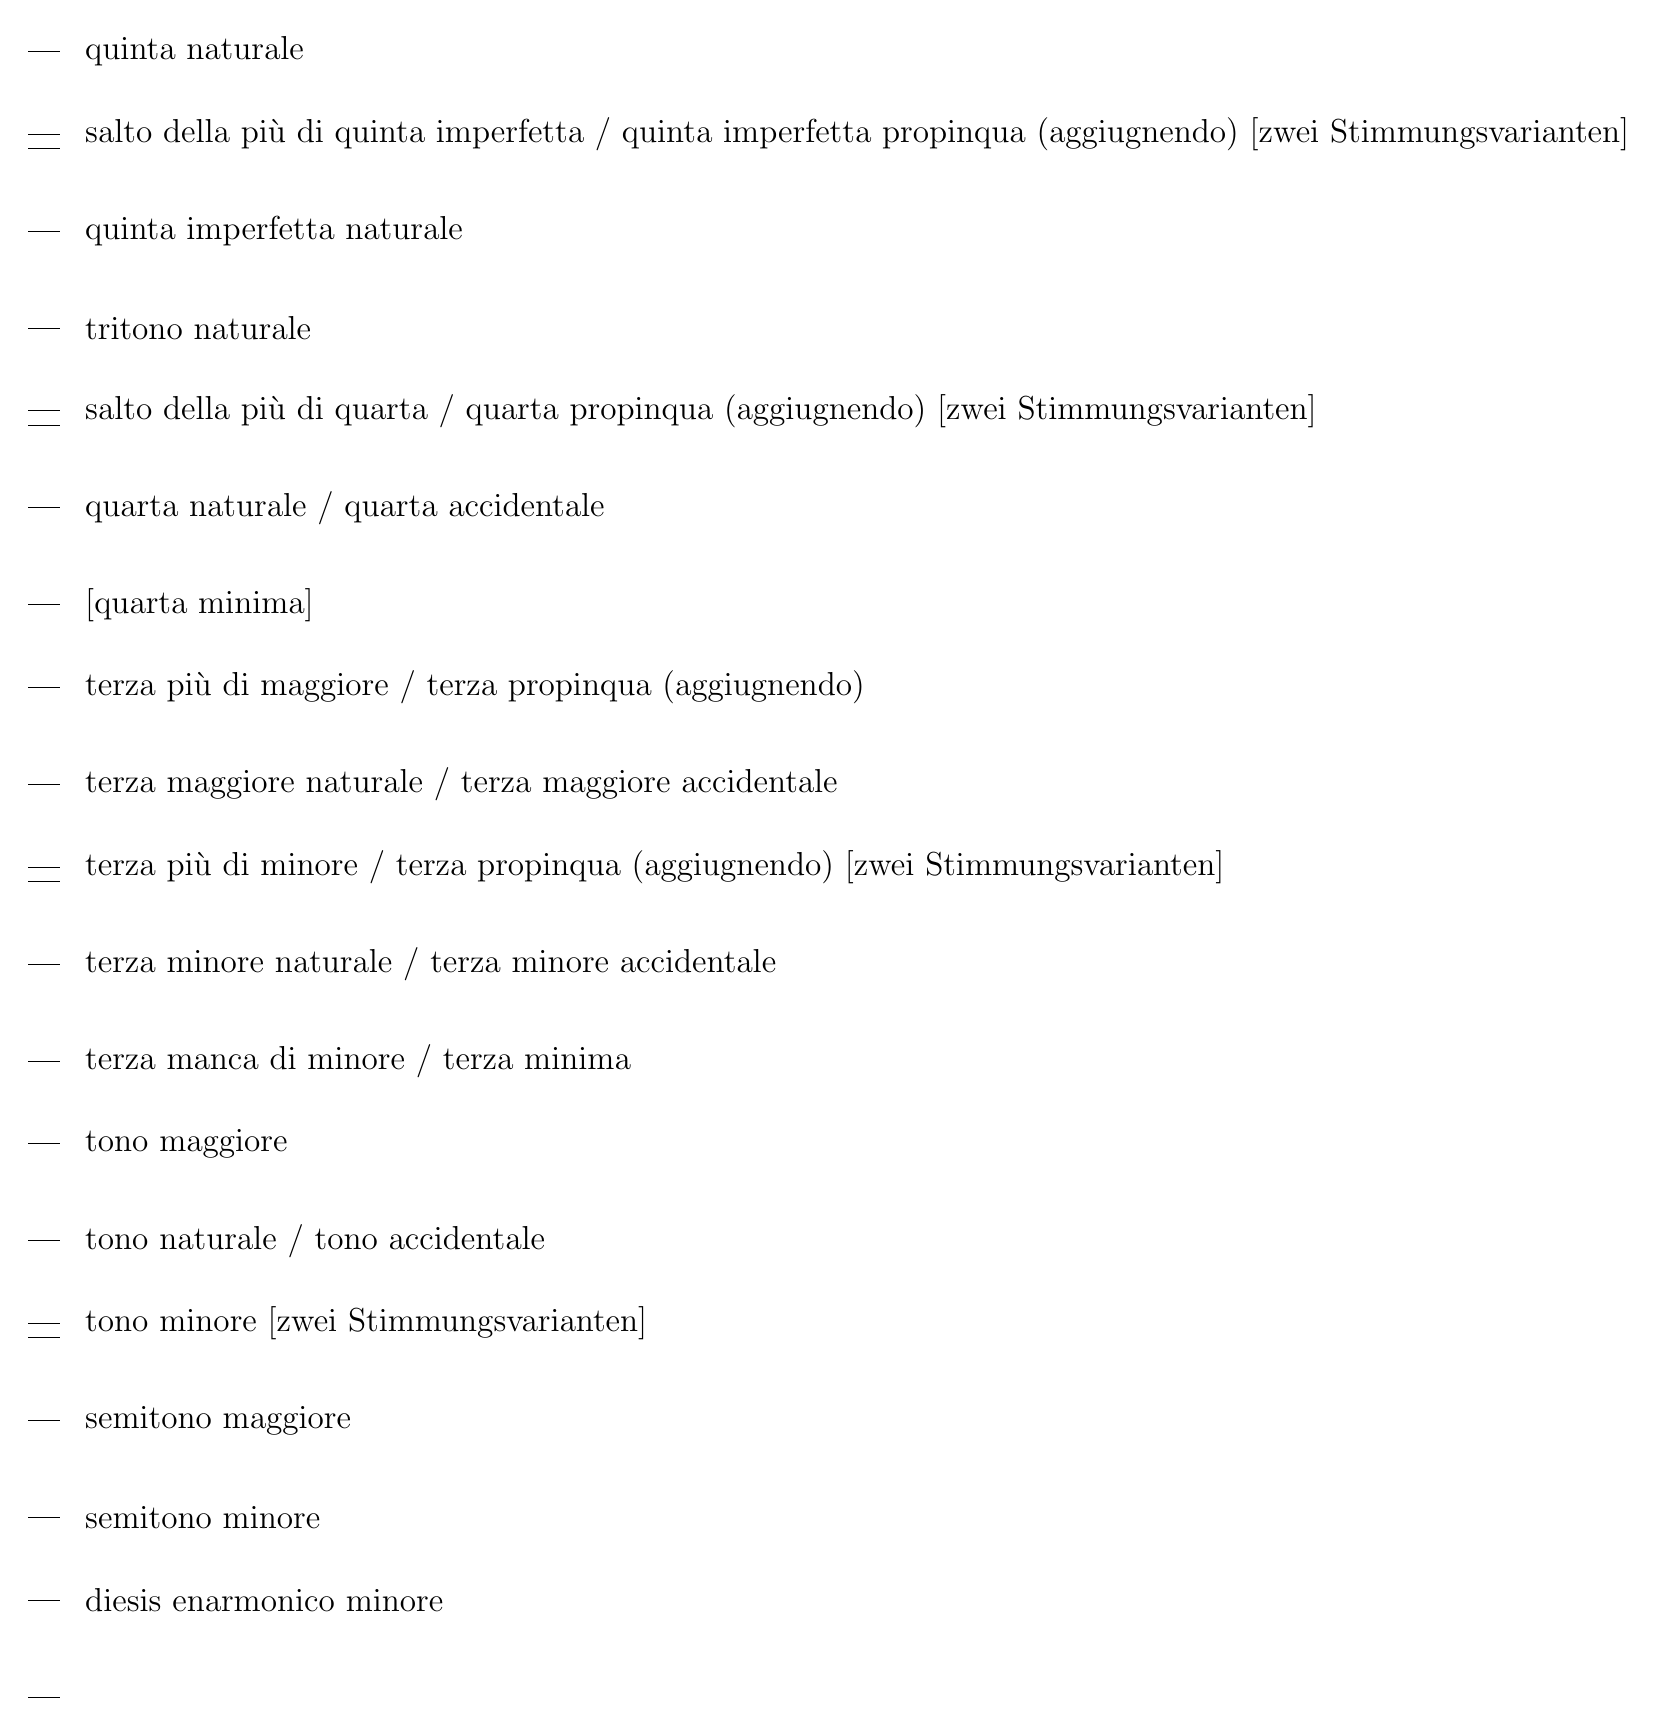
\begin{tikzpicture}

\node[anchor=west] at (145.79778, 1.2317159) { \large diesis enarmonico minore };
\node[anchor=west] at (145.79778, 2.2814996) { \large semitono minore };
\node[anchor=west] at (145.79778, 3.5132473) { \large semitono maggiore };
\node[anchor=west] at (145.79778, 4.7452087) { \large tono minore [zwei Stimmungsvarianten] };
\node[anchor=west] at (145.79778, 5.794632) { \large tono naturale / tono accidentale };
\node[anchor=west] at (145.79778, 7.026385) { \large tono maggiore };
\node[anchor=west] at (145.79778, 8.07611) { \large terza manca di minore / terza minima };
\node[anchor=west] at (145.79778, 9.307891) { \large terza minore naturale / terza minore accidentale };
\node[anchor=west] at (145.79778, 10.539737) { \large terza più di minore / terza propinqua (aggiugnendo) [zwei Stimmungsvarianten] };
\node[anchor=west] at (145.79778, 11.589268) { \large terza maggiore naturale / terza maggiore accidentale };
\node[anchor=west] at (145.79778, 12.821024) { \large terza più di maggiore / terza propinqua (aggiugnendo) };
\node[anchor=west] at (145.79778, 13.870781) { \large [quarta minima] };
\node[anchor=west] at (145.79778, 15.102524) { \large quarta naturale / quarta accidentale };
\node[anchor=west] at (145.79778, 16.334267) { \large salto della più di quarta / quarta propinqua (aggiugnendo) [zwei Stimmungsvarianten] };
\node[anchor=west] at (145.79778, 17.383963) { \large tritono naturale };
\node[anchor=west] at (145.79778, 18.615751) { \large quinta imperfetta naturale };
\node[anchor=west] at (145.79778, 19.848133) { \large salto della più di quinta imperfetta / quinta imperfetta propinqua (aggiugnendo) [zwei Stimmungsvarianten] };
\node[anchor=west] at (145.79778, 20.897165) { \large quinta naturale };
\draw (145.59778,0.0) -- (145.19778,0.0);
\draw (145.59778,1.2317159) -- (145.19778,1.2317159);
\draw (145.59778,2.2814996) -- (145.19778,2.2814996);
\draw (145.59778,3.5132473) -- (145.19778,3.5132473);
\draw (145.59778,4.5628123) -- (145.19778,4.5628123);
\draw (145.59778,4.7452087) -- (145.19778,4.7452087);
\draw (145.59778,5.794632) -- (145.19778,5.794632);
\draw (145.59778,7.026385) -- (145.19778,7.026385);
\draw (145.59778,8.07611) -- (145.19778,8.07611);
\draw (145.59778,9.307891) -- (145.19778,9.307891);
\draw (145.59778,10.357341) -- (145.19778,10.357341);
\draw (145.59778,10.539737) -- (145.19778,10.539737);
\draw (145.59778,11.589268) -- (145.19778,11.589268);
\draw (145.59778,12.821024) -- (145.19778,12.821024);
\draw (145.59778,13.870781) -- (145.19778,13.870781);
\draw (145.59778,15.102524) -- (145.19778,15.102524);
\draw (145.59778,16.15187) -- (145.19778,16.15187);
\draw (145.59778,16.334267) -- (145.19778,16.334267);
\draw (145.59778,17.383963) -- (145.19778,17.383963);
\draw (145.59778,18.615751) -- (145.19778,18.615751);
\draw (145.59778,19.665363) -- (145.19778,19.665363);
\draw (145.59778,19.848133) -- (145.19778,19.848133);
\draw (145.59778,20.897165) -- (145.19778,20.897165);
\end{tikzpicture}
\end{document}